%*******************************************************************************
%*********************************** Third Chapter *****************************
%*******************************************************************************

\chapter{Molecule VR Viewer}\label{chapter3}  %Title of the Third Chapter

This chapter describes all functionalities of the core and, simultaneously, result of presented work, which is the Molecule VR Viewer program. Description of methodology and implementation details are discussed in Chapter \ref{chapter4}.

Generally, Molecule VR Viewer is an application that presents structure of the molecule in Virtual Reality, basing on the data contained in PDB file. As the program provides several modes and options, functionalities are described step by step, starting from the main menu. For its full performance, application requires \textit{Oculus Rift} HMD with attached \textit{Leap Motion} device. 

%********************************** %First Section  **************************************
\section{Main Menu} %Section - 3.1 

As main menu window is created in 2D and requires keyboard and mouse input, it is not rendered for \textit{Oculus}. Starting panel is presented in Figure \ref{fig:mainmenu}.

\begin{figure}[h]
\centering    
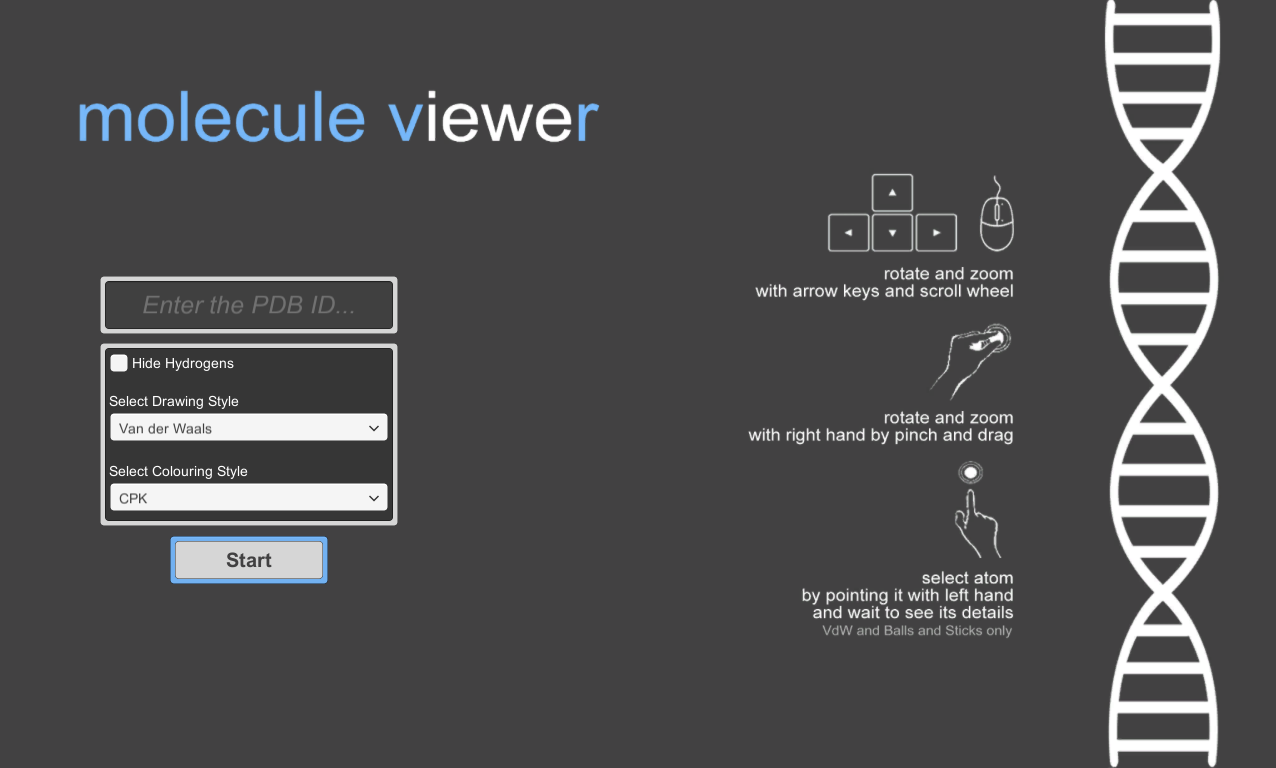
\includegraphics[width=1.0\textwidth]{Figs/mainmenu.png}
\caption{Starting window of the Molecule VR Viewer program.}
\label{fig:mainmenu} 
\end{figure} 

In the first input field, user is asked to enter the PDB ID- the four-character unique code that stands for a single molecule structure, which may be found in Protein Data Bank. Next, in settings panel, user may influence three properties of the generated visualisation. Toggle box "Hide Hydrogens" enables to choose whether to take hydrogen atoms into account while generating the structure or not. This function is purely practical, as the big number of hydrogen atoms (which often constitute around 50\% of the protein) may affect clarity of the view. However, if the PDB file does not provide data about hydrogen atoms (due to the method of obtaining the structure), toggle does not have any influence on the created view. Then, user may choose drawing and colouring style from the two drop down lists, but the choice of the representation style affects on the availability of colouring methods- for each drawing method different colouring settings may be applied. Application provides five different drawing settings: Van der Waals, Lines, Balls and Sticks, Ribbon and Backbone and four colouring styles: CPK, Residues, Subunits ans Secondary Structures. All of them are described in the following subsections.

On the right side of the menu window, short user's guide with pictograms presents the ways of rotating ad zooming the view, switching between modes and how to use the pointing mode.   

After clicking the "Start" button, correctness of the entered PDB ID is checked. In case of problems, error message occurs, allowing the user to recognize the problem. If the PDB code was found in the database, program presents "Wait..." message and analyses the selected structure to draw it. From this moment, user may put on the head-mounted display.
   
%********************************** %Second Section  **************************************
\section{Drawing Styles} %Section - 3.2

\subsection{Van der Waals}

Van der Waals representation creates for each atom a sphere of Van der Waals radius, which is different for every single element. It illustrates the imaginary volume that is occupied by the atom, in which it may interact with other atoms. When the atoms are bounded covalently, their Van der Waals spheres overlap. Thus, the representation shows the approximate shape of the whole molecule and its potentially accessible places, like active sites, which are highly important in case of ligands binding, their design etc. Example of such shape obtained with Molecule VR Viewer is shown in Figure \ref{fig:vdw}.

In addition to CPK colouring style presented in the example, Van der Waals drawing style enables Residues and Subunits colouring. 

\begin{figure}[!htb]
\centering    
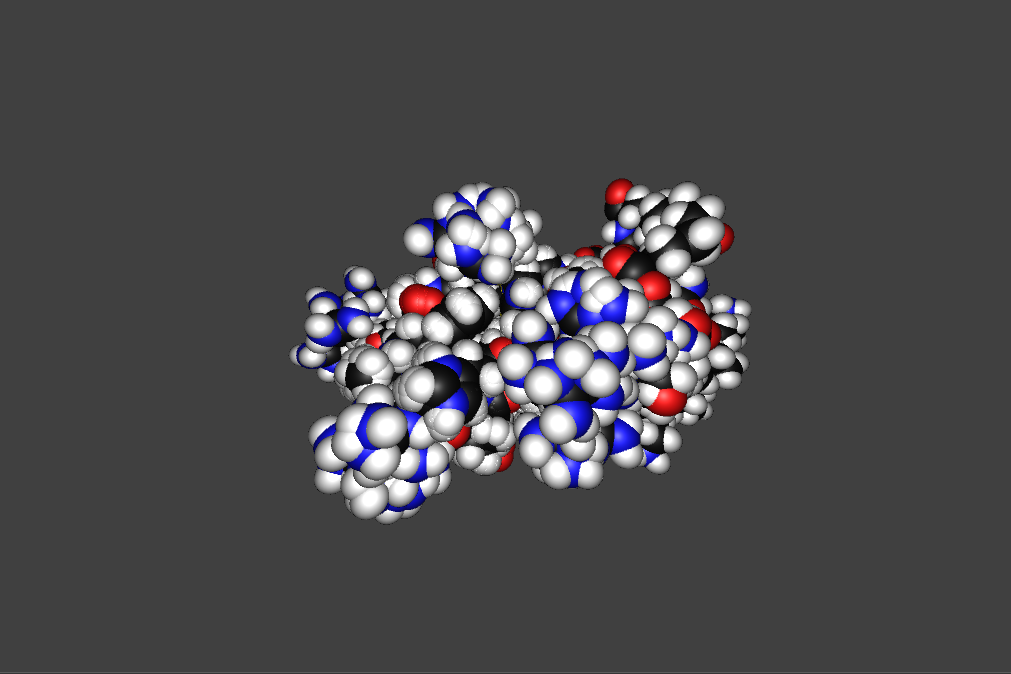
\includegraphics[width=0.8\textwidth]{Figs/vdw.png}
\caption{Van der Waals representation of yeast transcription factor ADR1 (PDB ID: 1ARD) with CPK colouring and showed hydrogens.}
\label{fig:vdw} 
\end{figure}

\subsection{Lines}
\begin{figure}[!htb]
\centering    
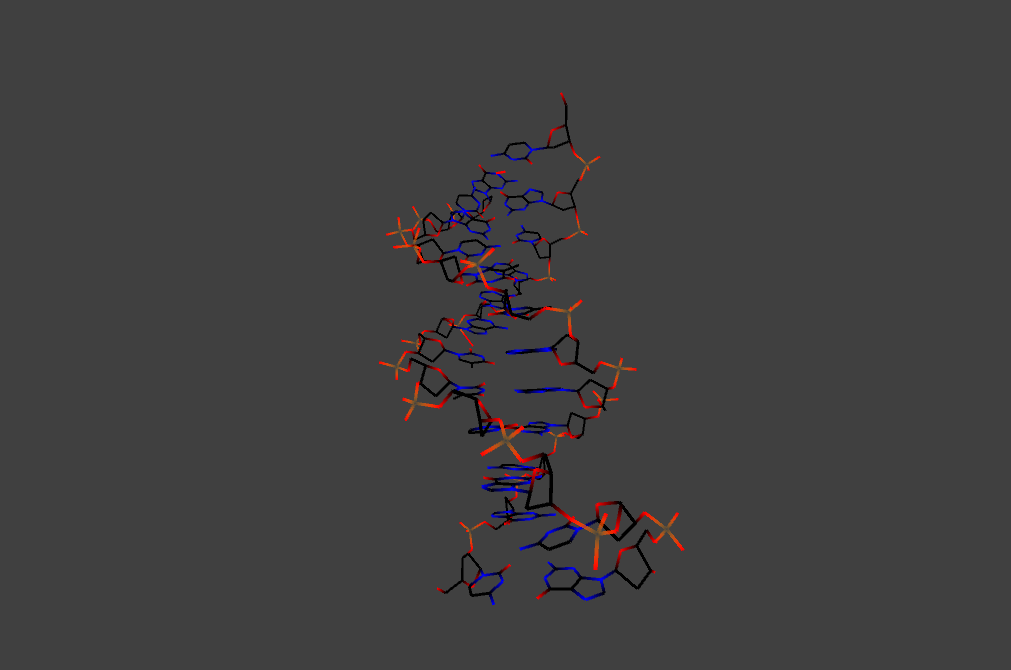
\includegraphics[width=0.8\textwidth]{Figs/lines.png}
\caption{Structure of the B-DNA dodecamer (PDB ID: 1BNA) obtained with Lines style and CPK colouring. The double helix structure of this nucleic acid is clearly visible, as well as belonging nucleobases.}
\label{fig:lines} 
\end{figure}

Another visualisation style is showing the covalent bonds existing in the structure and because of that is called Lines representation. Resulted wireframe is clear and, for the experienced scientist, easy to understand and to distinguish individual residues. Comparing to Van der Waals representation, Lines show the skeleton of the molecule, resulting in not crowded view, where one can easily find, for example, chemical rings. The exemplary structure made with bond diagram is presented in Figure  \ref{fig:lines}.

As shown, CPK colouring in this representation is made by smooth transition of colour between bonded atoms. The colouring options in this case are same as in Van der Waals setting.

\subsection{Balls and Sticks}

\begin{figure}[!htb]
\centering    
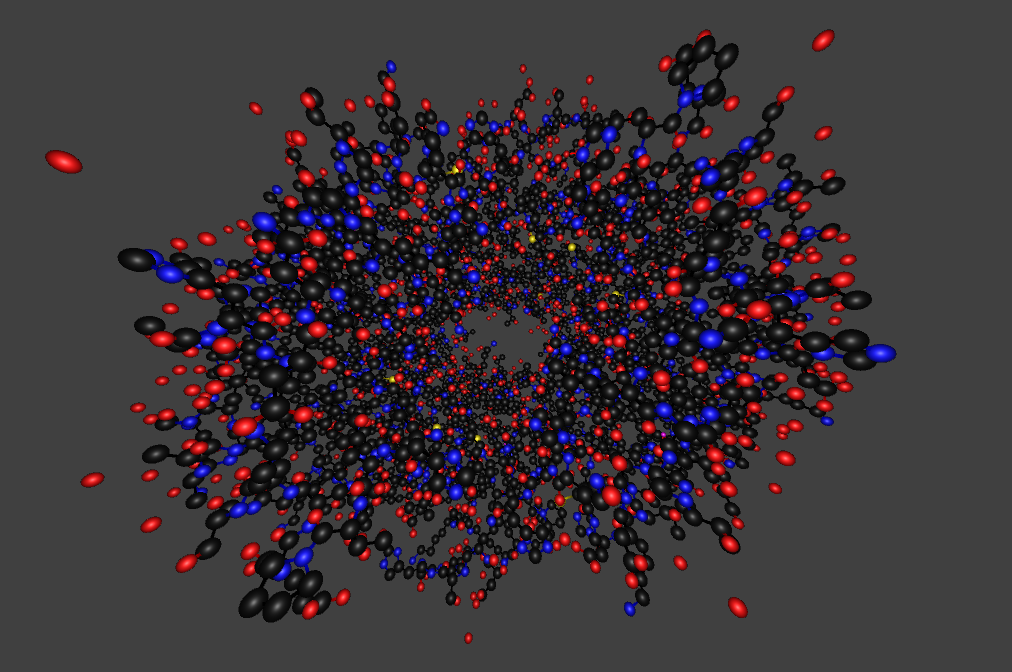
\includegraphics[width=0.8\textwidth]{Figs/balls.png}
\caption{Deoxy human hemoglobin (PDB ID: 1A3N) - important transporter of oxygen, shown with Balls and Sticks setting and CPK Colouring.}
\label{fig:balls} 
\end{figure}

Balls and Sticks is simply fusion of Lines and Van der Waals representation. To make the clear view, radii of the atoms are twice reduced. This drawing style is widely used in the molecule visualisation for better understanding, especially for education purposes. Nevertheless it is important to remember, that real atoms are not spheres bonded with sticks, and such idea is only a convention, which does not provide proper information about molecular shape. Illustration of Balls and Sticks representation demonstrates Figure \ref{fig:balls}. As the presented example is constituted by relatively big protein (tetramer- consists of four chains), the general view seems to be unclear. This case proves, that magnifying the view and looking around freely is crucial in the context of useful visualisation.


\subsection{Backbone}

As protein is, generally saying, chain of amino acids, which are connected with peptide bonds, it does have a main backbone trace. It is one of the most simplified type of representation and is obtained by omitting amino acid side chains. In case of protein, the backbone is created between alpha carbon atoms (carbon atom before the carbonyl carbon in peptide, which bonds with amino acid residues). What is more, nucleic acids are biopolymers as well, and their backbone is created by phosphate and deoxyribose molecules, and in simplified form- by linked phosphorus atoms.

This representation style puts emphasis on the secondary structure, ignoring the primary one somehow. In this approach is not the single residues that matters, but the structures that they form. Additionally, this drawing setting is great for showing the tertiary structure- protein geometric shape or even quaternary one- with all the subunits of molecule, as presented in Figure \ref{fig:backbone}. Because of all those properties, the only colouring method applicable here is the Subunits style.

\begin{figure}[!htb]
\centering    
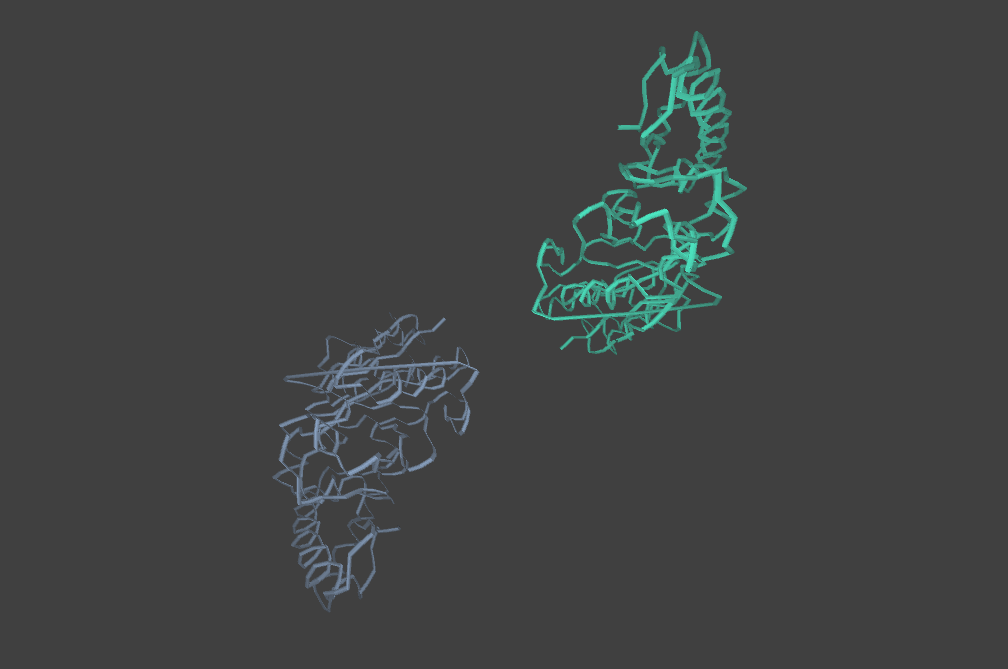
\includegraphics[width=0.8\textwidth]{Figs/backbone.png}
\caption{Papain dimer (PDB ID: 4QRV) presented in Backbone style with Subunits colouring. One can recognize alpha helix structures occurring in each chain.}
\label{fig:backbone} 
\end{figure}

\subsection{Ribbon}

The last drawing style supported by Molecule VR Viewer is Ribbon diagram. It is one of the most commonly used in both scientific and educational world, since it illustrates the whole organisation of protein structure. One can say, that it is improved Backbone representation, with even bigger emphasis put on secondary structure. It is achieved by presenting $\alpha$-helices and $\beta$-strands, the most common and important secondary structure types, as cylindrical spiral ribbons and arrows, respectively, both following the backbone of the peptide. $\beta$-sheet arrows, except just their distinguishing from other structures, play another important role- they show the direction of protein chain, from amino to the carboxyl end. These are the crucial elements of ribbon diagram and they are supported by Molecule VR Viewer, however, in more complex diagrams, other structures, such as loops, turns or even disulfide bonds may be presented. 

\begin{figure}[!htb]
\centering    
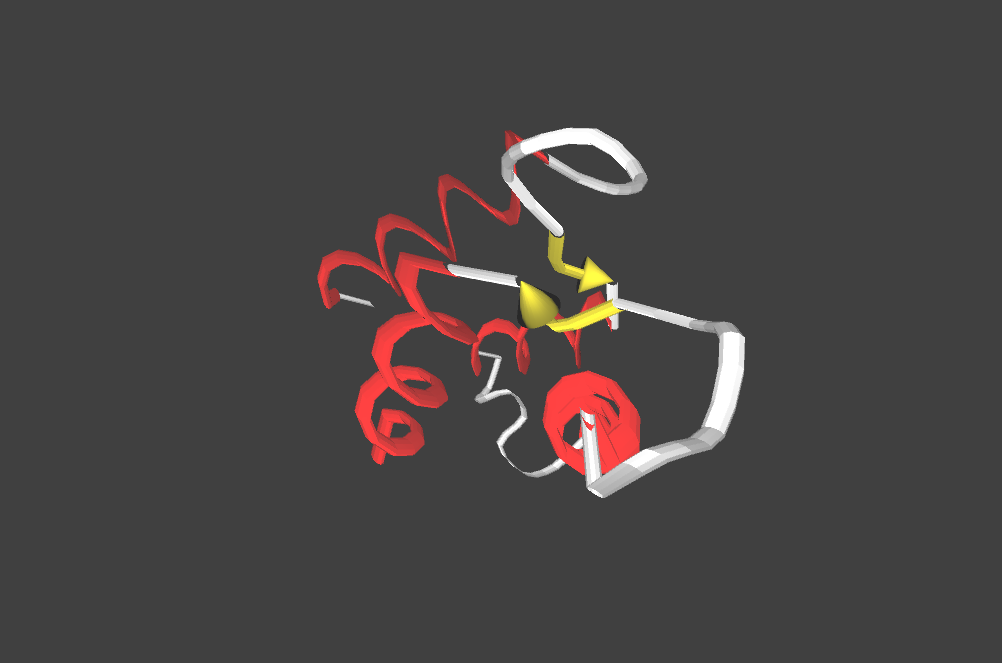
\includegraphics[width=0.8\textwidth]{Figs/ribbon.png}
\caption{Ribbon diagram of calbindin D9k from \textit{Bos Taurus} (PDB ID: 2BCA) with noticeable four $\alpha$-helices and two $\beta$-strands}
\label{fig:ribbon} 
\end{figure}

Exemplary protein visualised with Ribbon representation is shown in Figure \ref{fig:ribbon}. In this diagram the most useful colouring style was set- Secondary Structure. However, it is possible to apply Subunits colouring as well.

 


%********************************** %Third Section  **************************************
\section{Colouring styles} %Section - 3.3 
\subsection{CPK}
Colouring style called CPK from it's authors names (Corey, Pauling, Koltun) is a standard convention of colouring atoms on basis of elements they represent \cite{Koltun65}. As the original patent of Koltun does not mention all of the elements that may occur in biomolecules, they have been set for this work purposes, and the result is shown in Table \ref{tab:cpk}.

\begin{table}[h]
\centering 
\begin{tabular}{|r|c|}
  \hline 
  H & \cellcolor[rgb]{1,1,1} \\
  \hline
  C & \cellcolor[rgb]{0,0,0} \\
  \hline
  N & \cellcolor[rgb]{0,0,1} \\
  \hline
  O & \cellcolor[rgb]{1,0,0} \\
  \hline
  F, Cl & \cellcolor[rgb]{0,1,0} \\
  \hline  
  P, Fe & \cellcolor[RGB]{255, 153, 0} \\
  \hline
  S & \cellcolor[rgb]{1, 0.92, 0.016} \\
  \hline
  Br & \cellcolor[RGB]{153, 0, 0} \\
  \hline
  I & \cellcolor[RGB]{148, 0, 211} \\
  \hline
  Be, Mg, Ca, Sr, Ba, Ra & \cellcolor[RGB]{0, 102, 0} \\
  \hline
  Li, Na, K, Rb, Cs, Fr & \cellcolor[RGB]{159, 0, 255} \\
  \hline
  Ti & \cellcolor[rgb]{0.5, 0.5, 0.5} \\
   \hline
  other & \cellcolor[RGB]{255, 0, 227} \\
  \hline
\end{tabular}

\caption{CPK colour assignments used in Molecule VR Viewer.}
\label{tab:cpk}
\end{table}

The big advantage of this style is its clarity and the easiness of recognizing e.g. metal cofactors in metalloproteins. Such example is presented in the Figure \ref{fig:cpk}


\begin{figure}[!htb]
\centering    
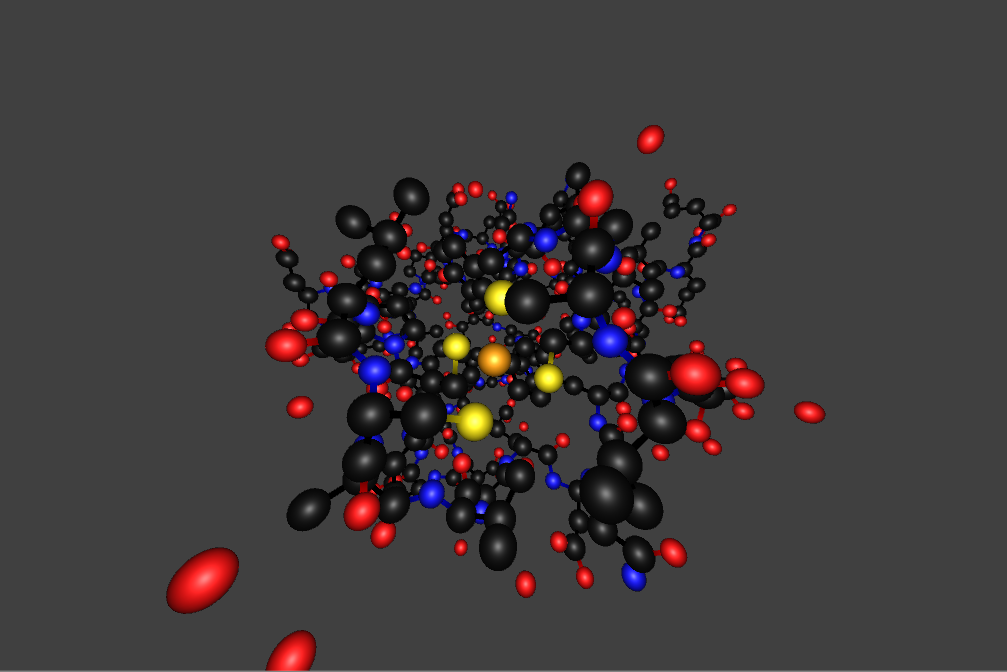
\includegraphics[width=0.8\textwidth]{Figs/cpk.png}
\caption{Fe$^{3+}$ ion (orange) in the binding pocket made out of 4 cysteine residues in the structure of rubredoxin (PDB ID: 1B2J) presented in CPK colouring mode and Balls and Sticks representation.}
\label{fig:cpk} 
\end{figure}

\subsection{Residues}

Both proteins and nucleic acid consist of meres- amino acids and nucleotides, respectively. Although, as mentioned before, experienced scientist may recognize the residue directly from its structure, it is more convenient to apply the distinguishing colouring style. Since there are 20 basic amino acids that build proteins, their colours were assigned following to the scheme presented in Table \ref{tab:residues}, which comes from the \textit{RasMol}, molecular visualisation program \cite{Rasmol16}. All of the other residue types have random color assigned. The example shows Figure \ref{fig:residues}.

\begin{table}[h]
\centering 
\begin{tabular}{|r|c|}
  \hline 
  ASP,GLU & \cellcolor[RGB]{230,10,10} \\
  \hline
   LYS,ARG & \cellcolor[RGB]{20,90,255} \\
  \hline
  PHE,TYR & \cellcolor[RGB]{50,50,170} \\
  \hline
  GLY & \cellcolor[RGB]{235,235,235} \\
  \hline
  ALA & \cellcolor[RGB]{200,200,200} \\
  \hline  
  HIS & \cellcolor[RGB]{130,130,210} \\
  \hline
  CYS, MET & \cellcolor[RGB]{230,230,0} \\
  \hline
  SER,THR & \cellcolor[RGB]{250,150,0} \\
  \hline
  ASN,GLN & \cellcolor[RGB]{0,220,220} \\
  \hline
  LEU,VAL,ILE & \cellcolor[RGB]{15,130,15} \\
  \hline
  TRP & \cellcolor[RGB]{180,90,180} \\
  \hline
  PRO & \cellcolor[RGB]{220,150,130} \\
   \hline
\end{tabular}

\caption{Amino acid colour assignments used in Molecule VR Viewer \cite{Rasmol16}.}
\label{tab:residues}
\end{table}

\begin{figure}[!htb]
\centering    
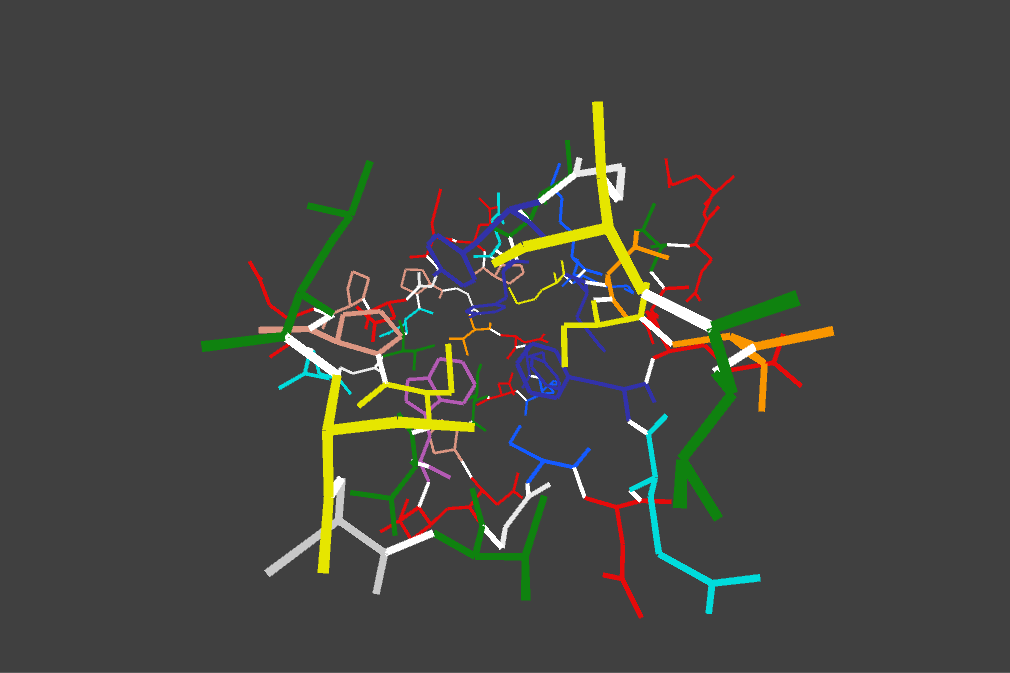
\includegraphics[width=0.8\textwidth]{Figs/residues.png}
\caption{The same rubredoxin (PDB ID: 1B2J) as in Figure \ref{fig:cpk}, presented with Residues colouring and Lines representation. In this case one can recognize 4 cysteine residues directly (yellow), not from the sulfur atoms.}
\label{fig:residues} 
\end{figure}

\subsection{Subunits}

Since protein or nucleic acid may be an assembly made of multiple chains, forming quaternary structure (in case of peptides), it is sometimes of high importance to recognize which atom belongs to which subunit, whether subunits are identical (homomers) or not (heteromers). Usually chains are named with consecutive letters of the alphabet, nevertheless, it is not a standard. Therefore, in Molecular VR Viewer, the colour of each subunit is assigned randomly, resulting in the image like in Figure \ref{fig:subunits}.

\begin{figure}[!htb]
\centering    
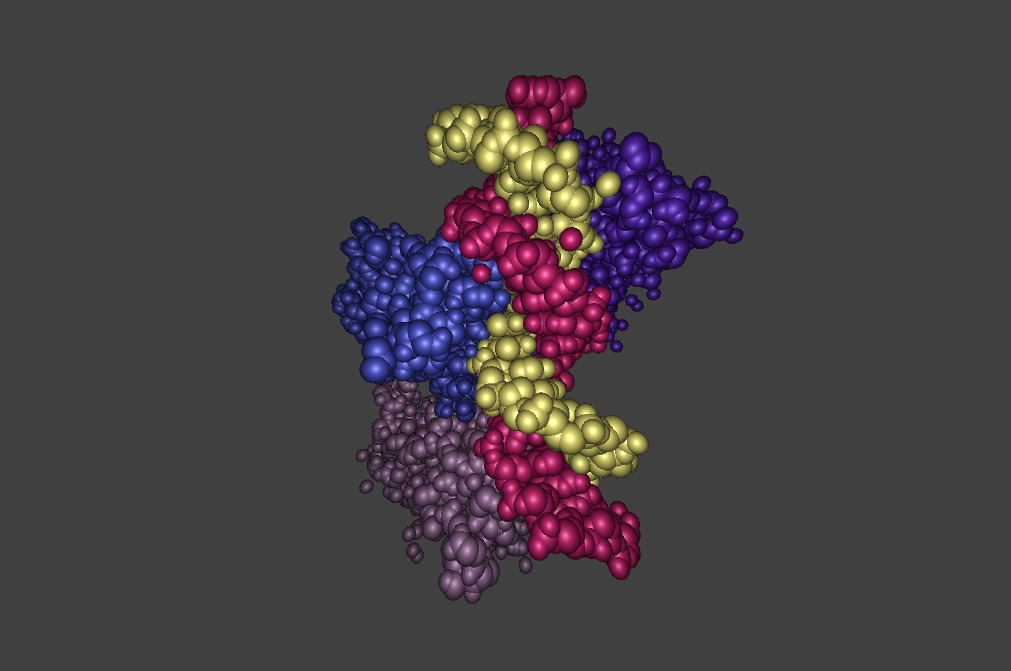
\includegraphics[width=0.8\textwidth]{Figs/subunits.png}
\caption{Tumor suppressor p53, which is of high interest in scientific world, complexed with DNA (PDB ID: 1TUP) presented with Subunits colouring and Van der Waals representation. It is not hard to distinguish two DNA chains (pink and yellow) forming double helix, from the protein units.}
\label{fig:subunits} 
\end{figure}

\subsection{Secondary Structures}
The last colouring setting, dedicated for Ribbon diagram, is the simplest one. As shown in Figure \ref{fig:ribbon}, each type of secondary structure has different colour assigned. $\alpha$-helices are red, $\beta$-sheets are yellow and the rest of the backbone is white. This style intensifies the effect of distinguishing secondary structures introduced in Ribbon drawing style.

%********************************** %Fourth Section  **************************************
\section{Visualisation Scene} %Section - 3.4

After clicking the "Start" button, required structure is loaded and user may start to watch and explore it. At the beginning, the molecule spins around its center, what may be stopped by pressing any key or what stops automatically after 15 seconds. Moreover, the name of presented molecule is displayed on the upper side of the user's view, which disappears after 15 seconds as well. With the \textit{Oculus} HMD on, user may look around this simulated nano-world.

\subsection{Rotating and Zoom}

Rotating and magnifying of the molecule is one of the most important feature for the properly designed visualization tool. In Molecule VR Viewer it may be accomplished in two ways. First one is simply pressing arrow keys on computer's keyboard for rotation up-down and left-right or scrolling the mouse wheel for zooming in and out. Nevertheless, with a head-mounted display on, user may find pressing the proper key hard, as the \textit{Oculus} headset does not provide transparency and the whole vision is covered with VR. Therefore, the second way is introduced.

Rotating and zooming of the image may be obtained by the Leap Motion Controller, the device already described in subsection \ref{leapmotion}. If it is attached to the HMD, it requires only to extend right arm forward. Then, on the viewer scene the hand model should appear, which is the exact equivalent of the user real hand.

To start moving the scene, user needs to make a pinch gesture (with index finger and thumb). Without releasing it, movement of the hand up-down and left-right rotates the molecule. For zooming in, user should pinch and pull it to yourself, for zooming out- pinch and push forward. The hand model making pinch gesture on the Molecular VR Viewer scene illustrates Figure \ref{fig:pinch}.    

\begin{figure}[!htb]
\centering    
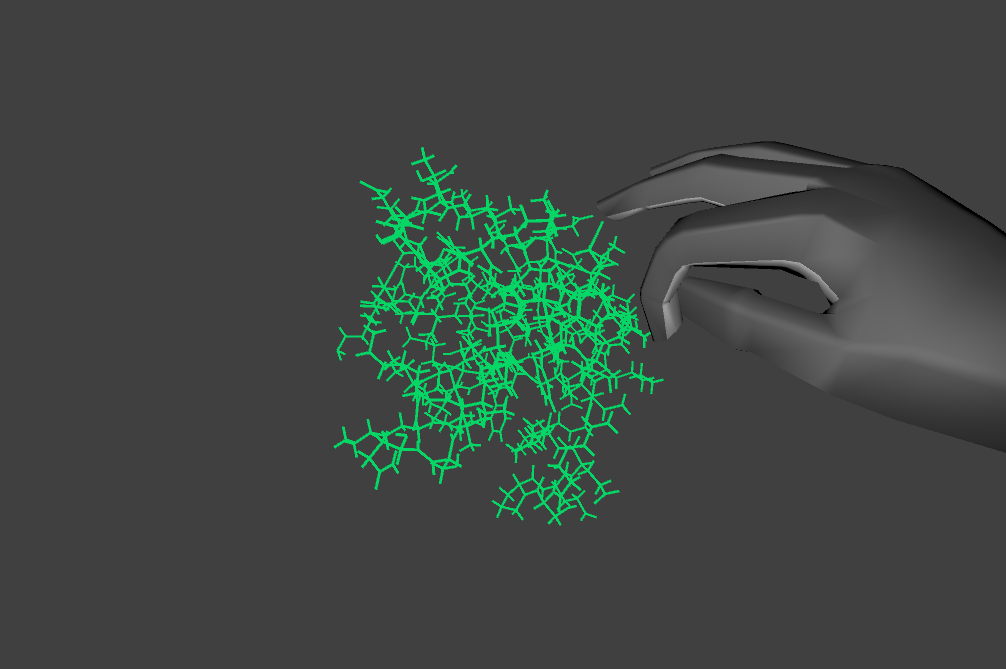
\includegraphics[width=0.8\textwidth]{Figs/pinch.png}
\caption{Pinching gesture enables rotation and magnifying of the structure.}
\label{fig:pinch} 
\end{figure}

Manipulating with \textit{Leap Motion} usage requires a bit of practice. However, this solution is perfect for the Virtual Environment, since it provide another dimension of user's immersion.

\subsection{Selecting mode}

In the 3D VR world, traditional, two-dimensional pointers (like computer mouse) do not find an application, obviously due to the lack of one dimension. However, in desktop programs for molecular visualisation, user has the ability of selecting single atom and checking its details. As the new solution should not be less functional, Molecule VR Viewer has another feature that solves this problem. The selecting mode with usage of \textit{Leap Motion} constitutes the solution.

\begin{figure}[!htb]
\centering    
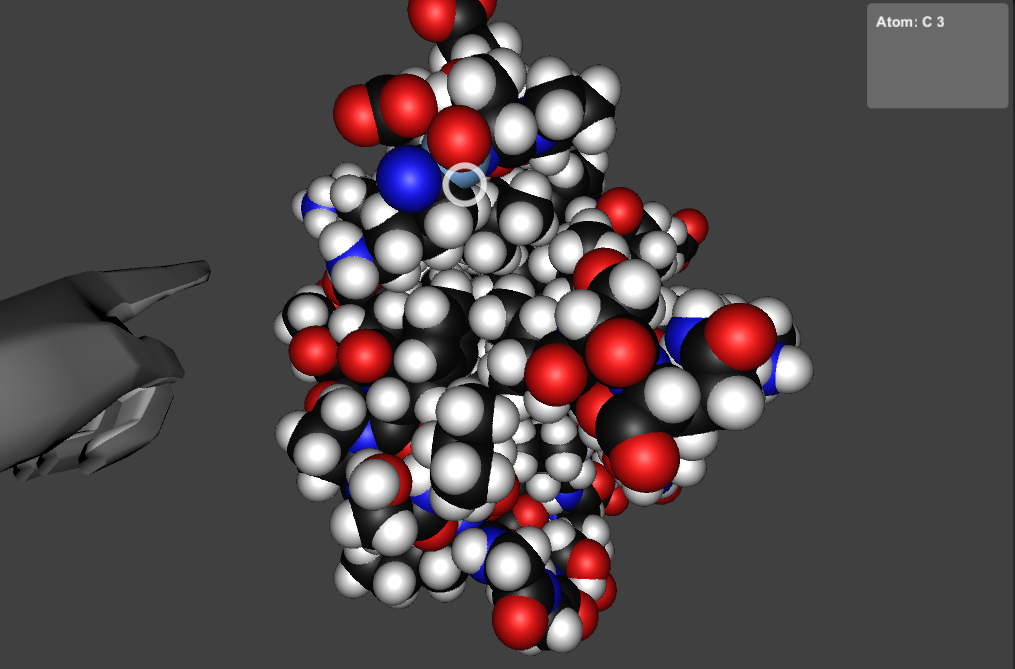
\includegraphics[width=0.8\textwidth]{Figs/pointing.png}
\caption{Pointing with the left hand at the atom. As seen, the cross hair is aimed at the carbon atom number 3, what changed the colour of the sphere from black to bright blue.}
\label{fig:pointing} 
\end{figure}

Since this feature is mostly needed for pointing on an atom, it is available only for Van der Waals and Balls and Sticks representations, as these are the only modes that in fact create objects for each atom. After loading a structure in one of these two styles, user may turn on the Selecting mode by extending left arm forward. In other cases, the left hand does not appear on the screen and the mode is inactive.

Selecting is held by pointing with an index finger at the chosen atom. Pointed sphere changes its color to the bright blue and the atom's name and number is displayed in the right upper corner. That feature enables searching for the requested fragment. If user wants to become familiar with details of the chosen atom, he or she should point at it for few seconds. Targeting is facilitated by a cross hair, which is simultaneously a progress bar indicating the time that left for the atom details presentation (Figure \ref{fig:pointing}). The time buffer protects the user from accidental pointing on other atoms, which could cause chaotic performance.
After successful selection of an atom, its name, element, number, residue and chain is displayed in the upper right corner for 5 seconds (Figure \ref{fig:selecting}). In this time user cannot select another sphere. 

Escaping from the selecting mode is possible by hiding left hand out of \textit{Leap Motion} controller's vision. 

\begin{figure}[!htb]
\centering    
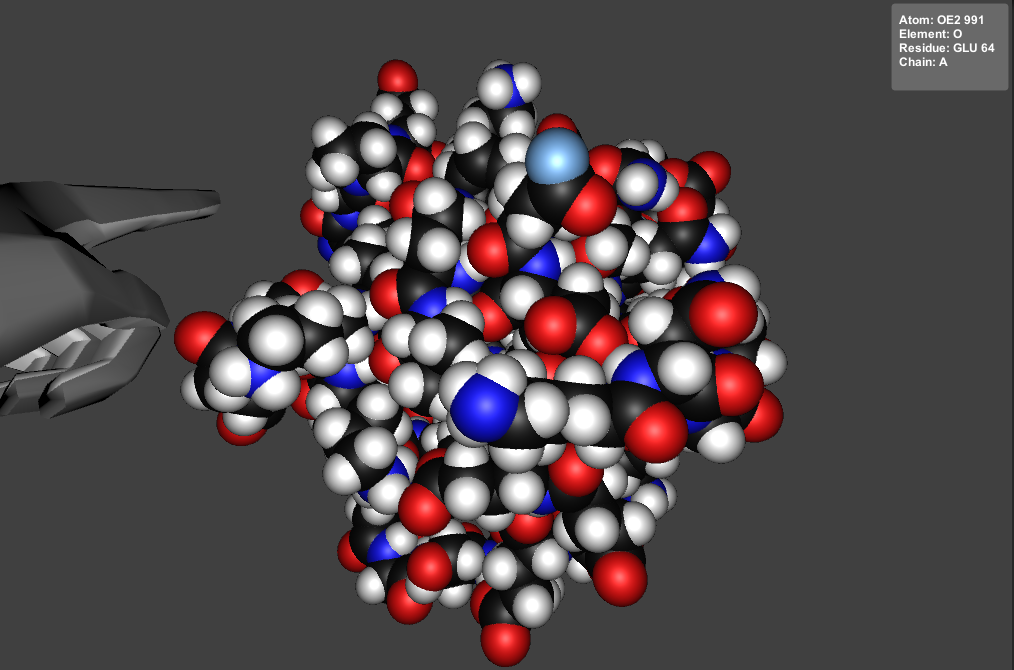
\includegraphics[width=0.8\textwidth]{Figs/selecting.png}
\caption{Selected atom and its details shown in the right upper corner. The cross hair is hidden, as time needed for details presentation has passed and pointing at other atoms is temporarily inactive.}
\label{fig:selecting} 
\end{figure}

\subsection{Exit}

As the re-typing of PDB ID code etc. requires taking off the HMD, there is no way to get back to main menu in single session. Changing of molecule code or chosen setting requires restarting of the program. 

Closing the Molecule VR Viewer may be done by simply clicking the escape key on the keyboard. 

